\documentclass{article}
\usepackage[utf8]{inputenc}
\usepackage{pgfplots}
\usepackage{array}
\usepackage{enumitem}
\usepackage{fancyhdr}
\usepackage{amssymb}
\usepackage{verbatim}
\usepackage{fancyvrb}
\usepackage{listings}
\usepackage{mathtools}
\usepackage{qtree}
\usepackage{graphicx}

\DeclarePairedDelimiter\floor{\lfloor}{\rfloor}
\setlength\parindent{0pt}

\pgfplotsset{compat=1.11, width=12cm, height=9cm}

\usepackage{xcolor}
\definecolor{codegreen}{rgb}{0,0.6,0}
\definecolor{codegray}{rgb}{.5,.5,.5}
\definecolor{codepurple}{rgb}{.58,0,.82}
\definecolor{backcolor}{rgb}{1,1,1}

\lstdefinestyle{Pseudocode} {
    backgroundcolor=\color{backcolor},
    commentstyle=\color{codegreen},
    keywordstyle=\color{magenta},
    numberstyle=\tiny\color{codegray},
    stringstyle=\color{codepurple},
    breakatwhitespace=false,
    breaklines=true,
    captionpos=b,
    keepspaces=false,
    numbers=left,
    numbersep=5pt,
    showspaces=false,
    showstringspaces=false,
    showtabs=false,
    tabsize=2
}

\graphicspath{ {./images/} }

\title{Final Report}
\author{Ishmam Kabir and Troy Witmer}
\date{2025-05-01}

\begin{document}
\maketitle

\section{Objective}
Our inital Objective was to use openars to predict future data points on a candlestick graph based
on historical data.
This uses open, high low, and close data points on each candlestick to predict the next few.
This project uses stock data because of its historical availability, accuracy.
However due to unforeseen circumstances we could not implement all candlestick
data such as high, low, and open, instead we settled for close and changed from a
candlestick graph to a line graph. Due to errors in the python version of OpenNARS our
program was cut short and was not able to be fully implemented.

\section{Problems}

During our development we ran into two big problems, first was the prediction rate vs
the rate we were sending data to NARS, second was the babbling feature was the only
data we were receiving due to issues in the source code. These problems appeared to
be seperate at first with our minds focusing on figuring out how we could get NARS to
execute a sensorimotor command everytime we sent a sentence to it. After hours of
failing to come up with a solution we stumbled across the source code for the SensorimotorChannel
which contained bypasses, which according to the comments stated an issue with the Reasoner.
After much time debugging, we were unable to find a fix for the issue. As a result of
the Reasoner being broken all commands sent from the SensorimotorChannel were random due
to the babbling feature.

\vspace{3mm}
Here is snippits found inside the source code of OpenNARS Python.

\begin{lstlisting}[style=Pseudocode, mathescape=true]
// cheating
// since something is wrong the reasoner, such that it cannot generate sub-goals correctly, I have to cheat.

reactions, ret = self.input_buffer.buffer_cycle(inputs, memory)
for each in reactions:
  self.reactions.push(each, self.reaction_evaluation(each, memory))

return ret
// original
// return self.input_buffer.buffer_cycle(inputs, memory)


// cheating
// since something is wrong the reasoner, such that it cannot generate sub-goals correctly, I have to cheat.
// this means there are reactions with no corresponding goals
if reaction.goal is None:
    return 0.7

\end{lstlisting}

\section{Method and Results}
Despite the issues we still wrote most of the code required to complete our Objective.

\subsection*{Sentence Building}
In order to communicate with NARS we constructed sentences relating to the price of closing
for that iteration. when NARS's prediction was within a buffer value. To begin with we
created the relation for when NARS was in the buffers range:

\begin{lstlisting}
msg = "<{SELF} --> [good]>. %1;0.9%"
\end{lstlisting}

If NARS fell below the true close then we computed the following:
\begin{lstlisting}
msg_1 = "<{up} --> [on]>. %1;0.9%"

f = str(percent_correct(cur_predicted, expected))

msg_2 = "<{SELF} --> [good]>. %" + f + ";0.9%"
\end{lstlisting}

If NARS was above the true close then we computed the following:
\begin{lstlisting}
msg_1 = "<{down} --> [on]>. %1;0.9%"

f = str(percent_correct(cur_predicted, expected))

msg_2 = "<{SELF} --> [good]>. %" + f + ";0.9%"
\end{lstlisting}

To calculate an f value that was meaningful for NARS we decided to use a formula for
percent correctness bounded between 0 and 1. If the observed value was far away from
the true value then the function would return a low f value. If the observed was
close to the true value then f would be closer to 1, telling NARS that it was "close"
to what the truth was.
\begin{lstlisting}[style=Pseudocode, mathescape=true]
def percent_correct(true, observed):
    if true == 0:
        return 1.0 if observed == 0 else 0.0
    error = abs(observed - true) / abs(true)
    return max(0.0, 1 - error)
\end{lstlisting}

Our ideal scenario would include obtaining at least one sensorimotor command everytime we
sent a sentence to NARS, more if its prediction was way off. Doing so would have allowed us
to only have to increment the predicted value of NARS by one per command.

\vspace{3mm}
Here is a graph depicting our failure, the only movement is from babbling with an augmentation
of NARS's predicted value set to 100
\begin{center}
	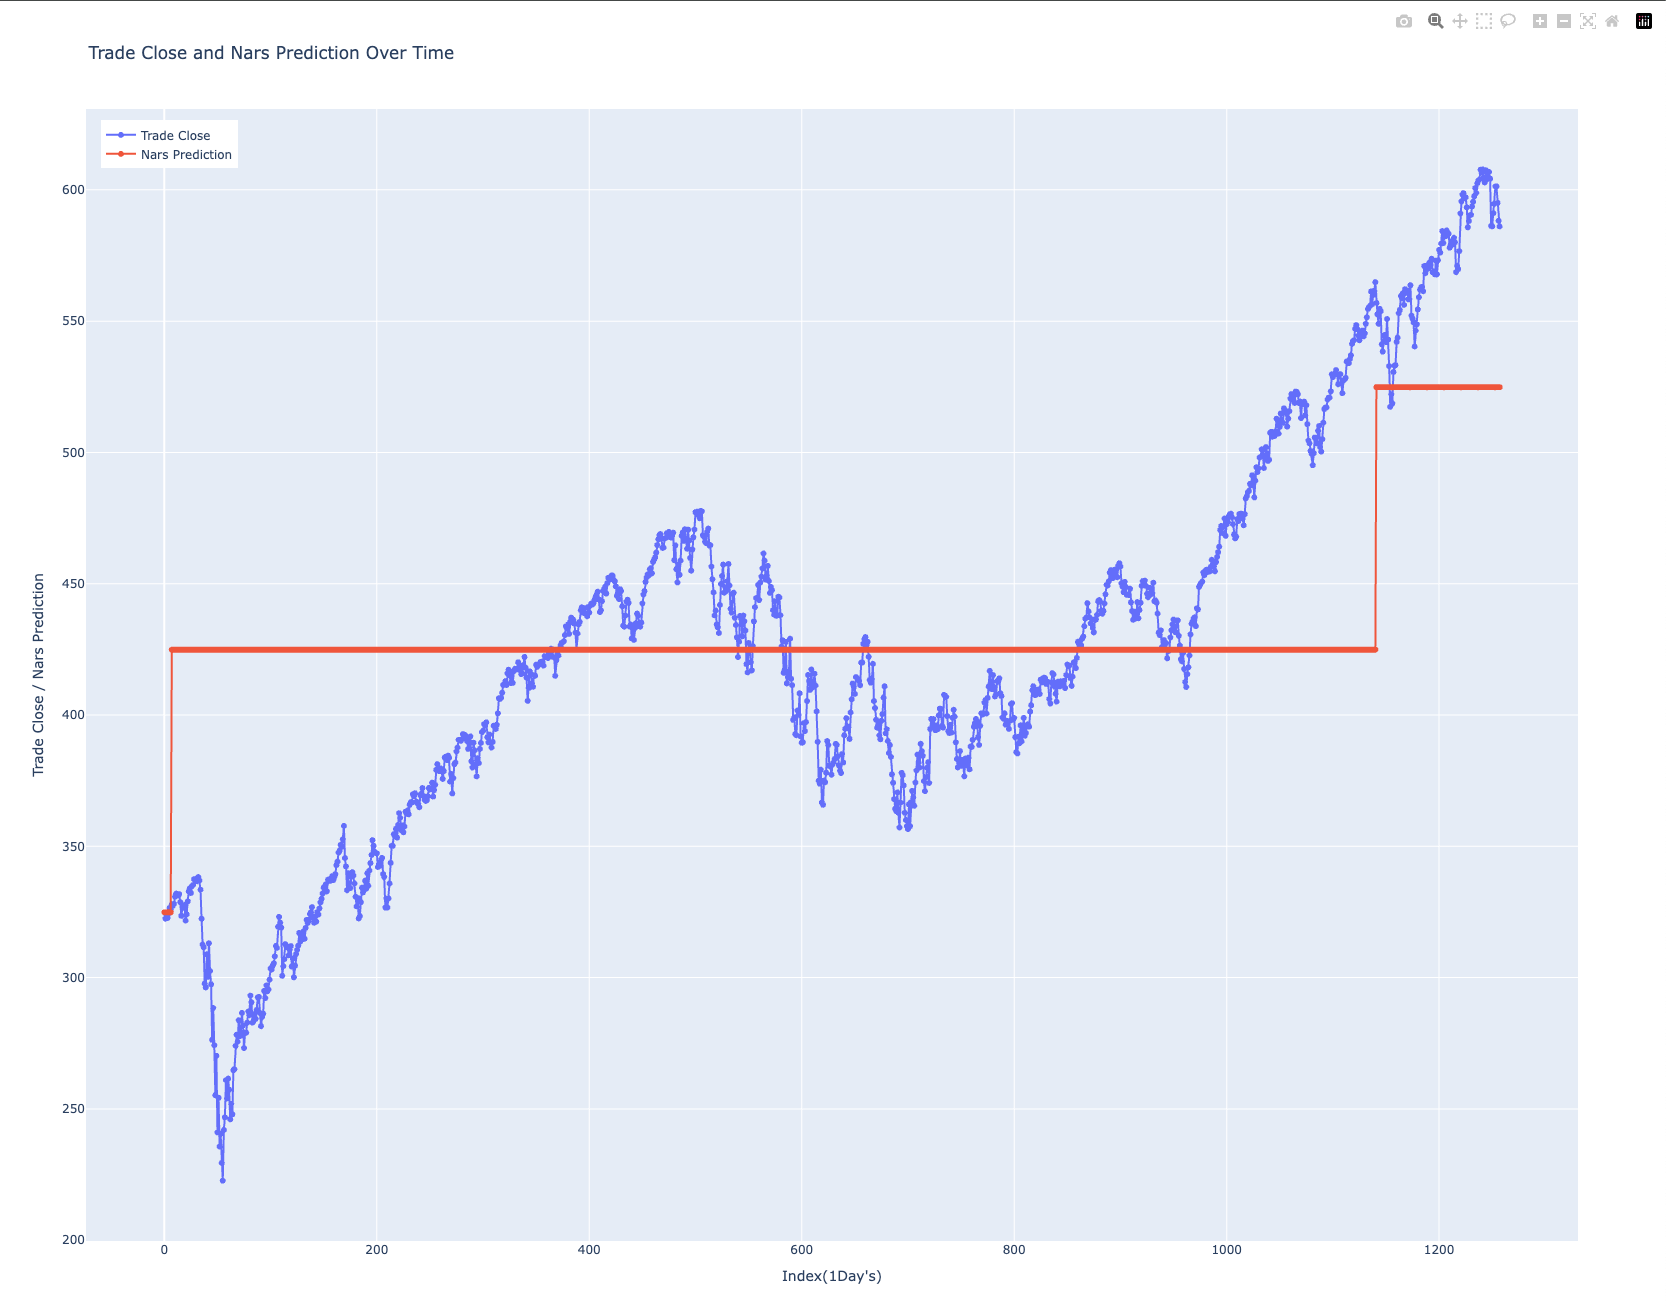
\includegraphics[width=\textwidth]{screenshot.png}
\end{center}

All our candlestick data was obtained via Alpaca API.
\end{document}

